\documentclass[
  bibliography=totoc,     % Literatur im Inhaltsverzeichnis
  captions=tableheading,  % Tabellenüberschriften
  titlepage=firstiscover, % Titelseite ist Deckblatt
]{scrartcl}

% Paket float verbessern
\usepackage{scrhack}

% Warnung, falls nochmal kompiliert werden muss
\usepackage[aux]{rerunfilecheck}

% unverzichtbare Mathe-Befehle
\usepackage{amsmath}
% viele Mathe-Symbole
\usepackage{amssymb}
% Erweiterungen für amsmath
\usepackage{mathtools}

% Fonteinstellungen
\usepackage{fontspec}
% Latin Modern Fonts werden automatisch geladen
% Alternativ:
%\setromanfont{Libertinus Serif}
%\setsansfont{Libertinus Sans}
%\setmonofont{Libertinus Mono}
\recalctypearea % Wenn man andere Schriftarten gesetzt hat,
% sollte man das Seiten-Layout neu berechnen lassen

% deutsche Spracheinstellungen
\usepackage{polyglossia}
\setmainlanguage{german}


\usepackage[
  math-style=ISO,    % ┐
  bold-style=ISO,    % │
  sans-style=italic, % │ ISO-Standard folgen
  nabla=upright,     % │
  partial=upright,   % ┘
  warnings-off={           % ┐
    mathtools-colon,       % │ unnötige Warnungen ausschalten
    mathtools-overbracket, % │
  },                       % ┘
]{unicode-math}

% traditionelle Fonts für Mathematik
\setmathfont{Latin Modern Math}
% Alternativ:
%\setmathfont{Libertinus Math}

\setmathfont{XITS Math}[range={scr, bfscr}]
\setmathfont{XITS Math}[range={cal, bfcal}, StylisticSet=1]

% Zahlen und Einheiten
\usepackage[
  locale=DE,                   % deutsche Einstellungen
  separate-uncertainty=true,   % immer Fehler mit \pm
  per-mode=symbol-or-fraction, % / in inline math, fraction in display math
]{siunitx}

% chemische Formeln
\usepackage[
  version=4,
  math-greek=default, % ┐ mit unicode-math zusammenarbeiten
  text-greek=default, % ┘
]{mhchem}

% richtige Anführungszeichen
\usepackage[autostyle]{csquotes}

% schöne Brüche im Text
\usepackage{xfrac}

% Standardplatzierung für Floats einstellen
\usepackage{float}
\floatplacement{figure}{htbp}
\floatplacement{table}{htbp}

% Floats innerhalb einer Section halten
\usepackage[
  section, % Floats innerhalb der Section halten
  below,   % unterhalb der Section aber auf der selben Seite ist ok
]{placeins}

% Seite drehen für breite Tabellen: landscape Umgebung
\usepackage{pdflscape}

% Captions schöner machen.
\usepackage[
  labelfont=bf,        % Tabelle x: Abbildung y: ist jetzt fett
  font=small,          % Schrift etwas kleiner als Dokument
  width=0.9\textwidth, % maximale Breite einer Caption schmaler
]{caption}
% subfigure, subtable, subref
\usepackage{subcaption}

% Grafiken können eingebunden werden
\usepackage{graphicx}
% größere Variation von Dateinamen möglich
\usepackage{grffile}

% schöne Tabellen
\usepackage{booktabs}

% Verbesserungen am Schriftbild
\usepackage{microtype}

% Literaturverzeichnis
\usepackage[
  backend=biber,
]{biblatex}
% Quellendatenbank
\addbibresource{lit.bib}
\addbibresource{programme.bib}

% Hyperlinks im Dokument
\usepackage[
  unicode,        % Unicode in PDF-Attributen erlauben
  pdfusetitle,    % Titel, Autoren und Datum als PDF-Attribute
  pdfcreator={},  % ┐ PDF-Attribute säubern
  pdfproducer={}, % ┘
]{hyperref}
% erweiterte Bookmarks im PDF
\usepackage{bookmark}

% Trennung von Wörtern mit Strichen
\usepackage[shortcuts]{extdash}

\author{%
  Dag-Björn Hering%
  \texorpdfstring{%
    \\%
    \href{mailto:authorA@udo.edu}{mark.schoene@udo.edu}
  }{}%
  \texorpdfstring{\and}{, }%
  Henning Ptaszyk%
  \texorpdfstring{%
    \\%
    \href{mailto:authorB@udo.edu}{henning.ptaszyk@udo.edu}
  }{}%
}
\publishers{TU Dortmund – Fakultät Physik}


\subject{V - 59}
\title{Modulation und Demodulation}
\date{
  Durchführung: 09. Juli 2018
  \hspace{3em}
  Abgabe: \today
}

\begin{document}

\maketitle
\thispagestyle{empty}
\tableofcontents
\newpage

\section{Theorie}
\label{sec:Theorie}

\subsection*{Zielsetzung}
\label{subsec:zielsetzung}
In dem hier beschriebenen Versuch wird untersucht,
inwiefern die Molwärme von der Temperatur abhängt.
Dazu werden zunächst drei Modelle zur theoretischen Beschreibung
der Molwärme von Festkörpern diskutiert und weiterhin experimentelle
Untersuchungen von Kupfer angestellt.
Anhand der daraus gewonnen Erkenntnisse, wird die Konstante $\Theta_{\text{D}}$,
die Debye-Temperatur, sowohl theoretisch, anhand des Debye-Modells,
als auch mit Hilfe der Messwerte bestimmt.

\subsection{Klassisches Modell}
\label{subsec:klassisch}
Bei einer rein klassischen Betrachtung, wird jedem Atom pro Freiheitsgrad eine mittlere
Energie von $\sfrac{k_{\text{B}} T}{2}$ zugeordnet. Die Atome im dreidimensionalen
Festkörper sind auf drei Bewegungsrichtungen, also sechs Freiheitsgrade, eingeschränkt, sodass
ein Mol eine mittlere Wärmeenergie von
\begin{align}
	U = 3 k_{\text{B}} T \, N_{\text{L}} = 3 R T\label{eqn:t2}
\end{align}
besitzt. Dabei bezeichnet $N_{\text{L}}$ die
Lohschmidtsche Zahl und
$R$ die allgemeine Gaskonstante.
Um die spezifische Molwärme $C_{\text{V}}$ zu erhalten,
wird die Energie eines Mols (siehe Gleichung \eqref{eqn:t2})
nach der Temperatur $T$ abgeleitet.
Es ergibt sich also
\begin{align}
	C_{\text{V}} = \frac{\partial U}{\partial T}
	\bigg\vert_{\text{V}} = 3 \, R \, . \label{eqn:t3}
\end{align}

Dieses Ergebnis ist bekannt als das Dulong-Petit-Gesetz.
Aus \eqref{eqn:t3} wird klar, dass in der klassischen Theorie,
die Molwärme sowohl unabhängig von der Beschaffenheit des
Festkörpers, als auch der Temperatur ist.


\subsection{Einsteinsches Modell}
\label{subsec:einstein}
Im einsteinschen Modell wird, im Gegensatz zum klassischen
Modell, berücksichtigt, dass die Energie, mit
der die Atome im Festkörper Schwingen, quantisiert ist.
Ausgehend von einer festgelegten Kreisfrequenz $\omega$,
werden nur Energien der Form
\begin{align*}
	E_{n} = \hbar \omega n
\end{align*}
zugelassen. Wobei $n$ eine natürliche Zahl ist.
Diese möglichen Energiezustände sollen der Boltzmann-Statistik
folgen. Sodass der Energieerwartungswert für ein Atom durch
\begin{align}
	\langle u \rangle_{\text{Einstein}} = \frac{\sum^{\infty}_{n = 0}
	E_{n} e^{\frac{-E_{n}}{k_{\text{B}} T}}}{\sum^{\infty}_{n = 0}
	e^{\frac{-E_{n}}{k_{\text{B}} T}}} \label{eqn:5}
\end{align}

Damit ergibt sich dann für die Molwärme
\begin{align}
	C_{\text{V,Einstein}} = 3 R \frac{\hbar^{2} \omega^{2}}{k_{\text{B}}} \frac{1}{T^{2}}
	\frac{e^{\frac{\hbar \omega}{k_{\text{B}} T}}}{e^{\frac{\hbar \omega}{k_{\text{B}} T}} - 1}\label{eqn:t7}
\end{align}

Dabei gilt
\begin{align}
	\lim_{T \rightarrow \infty} C_{\text{V,Einstein}} = 3R \, . \label{eqn:t8}
\end{align}
Es lässt sich also erkennen, dass  für große Temperaturen
das einsteinsche Modell in das Klassische übergeht und für kleine Temperaturen
antiproportional zu $T^2$ verläuft.

\subsection{Debye-Modell}
\label{subsec:debye}
Zur besseren Beschreibung der Realität, wird im Debye-Modell,
nicht wie im Einsteinschen von einer konstanten Schwingungsfrequenz,
sondern mehreren ausgegangen.
Dazu wird eine Verteilungsfunktion $Z(\omega)$ eingeführt.
Diese beschreibt das Spektrum der Schwingungsfrequenzen.
Für die Molwärme gilt also
\begin{align}
	C_{\text{V}} = \frac{\mathrm{d}}{\mathrm{d}T}
	\int_{0}^{\omega_{\text{max}}} \mathrm{d}\omega Z(\omega)
	\frac{\hbar \omega}{e^{\frac{\hbar \omega}{k_{\text{B}} T} - 1}} \, . \label{eqn:t9}
\end{align}
Im allgemeinen ist $Z(\omega)$  beliebig kompliziert.
Allerdings, wird im Debye-Modell die Annahme getroffen,
dass die Phasengeschwindigkeit unabhängig von Frequenz wie
Ausbreitungsrichtung ist.
Auf diese Weise vereinfacht sich $Z(\omega)$ derart, dass
ausschließlich die Eigenschwingungen eines Würfels(Kantenlänge $L$)
auf einem Intervall $\left[ \omega, \omega + \mathrm{d}\omega \right]$
zu berücksichtigen sind.
Damit ergibt sich
\begin{align}
	Z(\omega) \mathrm{d}\omega =  \omega^{2} \frac{L^{3}}{2 \pi^{2}}
	\left( \frac{1}{v_{\text{l}}^{3}} +
	\frac{2}{v_{\text{tr}}^{3}} \right) \mathrm{d}\omega \, . \label{eqn:t10}
\end{align}

Mit der longitudinalen Phasengeschwindigkeit $v_{\text{l}}$
und der transversalen $v_{\text{tr}}$.
In einem aus $N_{\text{L}}$ Atomen zusammengesetzten Festkörper,
existieren im dreidimensionalen Raum $3N_{\text{L}}$ Eigenschwingungen.
Aufgrund dieser Begrenzung, ist es notwendig, dass eine
Frequenz $\omega_{\text{D}}$, welche die obere Schranke der auftretenden
Frequenzen darstellt, existiert.
Diese wird als Debye-Frequenz bezeichnet und lässt sich
aus dem Zusammenhang
\begin{align}
	\int_{0}^{\omega_{\text{D}}} \mathrm{d}\omega = 3 N_{\text{L}} \label{eqn:t11}
\end{align}
gewinnen.
Es ergibt sich damit
\begin{align}
	\omega_{\text{D}}^{3} = \frac{18 \pi^{2} N_{\text{L}}}{L^{3}}
	\frac{1}{\frac{1}{v_{\text{l}}^{3}} + \frac{2}{v_{\text{tr}}}} \, .\label{eqn:t12}
\end{align}

Mithilfe von Gleichung \ref{eqn:t9}, \ref{eqn:t10} und \ref{eqn:t12}
lässt sich die spezifische Wärmekapazität als
\begin{align}
	C_{\text{V, Debye}} = \frac{\mathrm{d}}{\mathrm{d}T} \frac{9 N_{\text{L}} \hbar}{\omega_{\text{D}}^{3}}
	= \int_{0}^{\omega_{0}} \mathrm{d}\omega \frac{\omega^{3}}{e^{\frac{\hbar \omega}{k_{\text{B}} T}} - 1} \label{eqn:t14}
\end{align}
schreiben.
Mit den Definitionen
\begin{align}
	x &:= \frac{\hbar \omega}{k_{\text{B}} T} \label{eqn:t15} \\
	\frac{\theta_{\text{D}}}{T} &:= \frac{\hbar \omega_{\text{D}}}{\k_{\text{B}} T} \label{eqn:t16}
\end{align}
wird der Ausdruck für die Wärmekapazität \ref{eqn:t14} zu
\begin{align}
	C_{\text{V, Debye}} = 9 R \left(\frac{T}{\theta_{\text{D}}})\right)^{3}
	\int_{0}^{\frac{\theta_{\text{D}}}{T}} \frac{x^{4} e^{x}}{\left( e^{x} - 1 \right)^{2}} \, . \label{eqn:t17}
\end{align}

Bei einer Betrachtung von \ref{eqn:t17} im Grenzwert sehr großer Temperaturen,
ergibt sich für $C_{\text{V}}$ wieder die Konstante $3R$.

Da die Wärmekapazität kubisch mit der Temperatur ansteigt, kann der Beitrag freier Elektronen, der linear mit $T$ anwächst, im Festkörper vernachlässigt werden. \cite{sample}

\section{Durchführung}
\label{sec:Durchführung}

\subsection{(a) Erzeugen einer amplitudenmodulierten Schwingung mit
Hilfe eines Ringmodulators(keine Trägerabstrahlung)}
\label{subsec:durchfuehrung_a}
Zur Amplitudenmodulation durch einen Ringmodulator wir ein Aufbau,
entsprechend des Schaltbildes in Abbildung \ref{fig:schaltung_a}, verwendet.
Anschließend wird ein Bild, das Modulationssignal sowie moduliertes
Signal im Zeitraum zeigt, am Oszillographen aufgenommen.
% 
% \begin{figure}
%   \centering
%   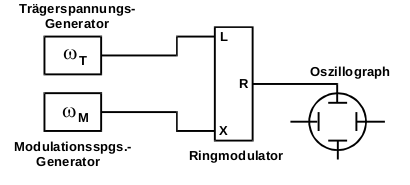
\includegraphics[width=0.7\textwidth]{figures/a_d.png}
%   \caption{Verwendete Schaltung zur Amplitudenmodulation mit Ringmodulator.\cite{sample}}
%   \label{fig:schaltung_a}
% \end{figure}


\subsection{(b) Untersuchung des Frequenzspektrums einer
amplitudenmodulierten Schwingung}
\label{subsec:durchfuehrung_b}
Um das Frequenzspektrum des in Abschnitt \ref{subsec:durchfuehrung_a} generierten
amplitudenmodulierten Signals zu untersuchen, wird in Abbildung
\ref{fig:schaltung_a} der Oszillograph durch einen Frequenzanalysator ersetzt.
Es wird ein Bild des Frequenzspektrums zwischen $\SI{324}{\hertz}$ und $\SI{1424}{\hertz}$
aufgenommen.


\subsection{(c) Erzeugen einer amplitudenmodulierten Schwingung
mit Hilfe einer Gleichrichterdiode (inklusive Trägerabstrahlung)}
\label{subsec:durchfuehrung_c}
Mit Hilfe der in Abbildung \ref{fig:schaltung_c} gezeigten Schaltung,
wird ein amplitudenmoduliertes Signal mit Trägerfrequenzabstrahlung erzeugt.
Das generierte Signal wird sowohl im Zeitbereich am Oszilloskop, als auch
im Frequenzbereich am Frequenzanalysator, dargestellt.

\begin{figure}
  \centering
  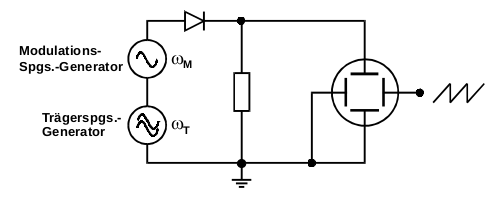
\includegraphics[width=0.7\textwidth]{figures/c_d.png}
  \caption{Verwendete Schaltung zur Amplitudenmodulation mit Diode.\cite{sample}}
  \label{fig:schaltung_c}
\end{figure}


\subsection{(d) Erzeugen einer frequenzmodulierten Schwingung}
\label{subsec:durchfuehrung_d}


\subsection{(e) Untersuchung der Phasenabhängigkeit eines
phasenempfindlichen Gleichrichters}
\label{subsec:durchfuehrung_e}


\subsection{(f) Demodulation einer amplitudenmodulierten Schwingung
mit Hilfe eines Ringmodulators}
\label{subsec:durchfuehrung_f}


\subsection{(g) Demodulation einer amplitudenmodulierten Schwingung
mit Hilfe einer Gleichrichterdiode}
\label{subsec:durchfuehrung_g}


\subsection{(h) Demoduolation einer frequenzmodulierten Schwingung
mit Hilfe eines Flankendemodulators}
\label{subsec:durchfuehrung_h}

\section{Auswertung}
\label{sec:Auswertung}

In der Tabelle \ref{tab:Messwerte} sind die Messwerte von
$R_{Probe}$ und $R_{Mantel}$ zur Messzeit $t$ aufgelistet.
Aus dem Zusammenhang
\begin{align}
  T=\num{0.00134} R_i^2 + \num{2.296} R_i - \num{30.1} \label{eqn:inKelvin}
\end{align}
kann aus den Messwerten der Widerständen
die Temperatur der Probe und
des Mantels errechnet werden, die ebenfalls in der
Tabelle \ref{tab:Messwerte} enthalten sind.
Die Abbildung \ref{fig:T_mess} zeigt den
Verlauf des Aufheizen sowohl von Probe
als auch des Mantels.



\begin{table}  % Messwerte
  \centering
  \caption{}
  \label{tab:Messwerte}
  \begin{tabular}{c c c c c}
  \toprule
  $t/\si{\second}$ & $R_{Probe}/\si{\ohm}$ & $T_{Probe}/\si{\kelvin}$ & $R_{Mantel}/\si{\ohm}$ & $T_{Mantel}/\si{\kelvin}$\\
  \midrule
  0	&	23.8	&	85.5	&	22.4	&	82.2   \\
  150	&	26.0	&	90.7	&	23.9	&	85.8   \\
  300	&	28.0	&	95.5	&	27.2	&	93.6   \\
  450	&	29.5	&	99.0	&	30.1	&	100.4   \\
  600	&	31.3	&	103.3	&	34.0	&	109.7   \\
  750	&	33.2	&	107.8	&	36.9	&	116.7   \\
  900	&	35.1	&	112.4	&	38.7	&	121.0   \\
  1050	&	37.0	&	116.9	&	40.1	&	124.3   \\
  1200	&	38.7	&	121.0	&	41.1	&	126.7   \\
  1350	&	40.3	&	124.8	&	42.2	&	129.4   \\
  1500	&	43.4	&	132.3	&	44.3	&	134.5   \\
  1800	&	46.2	&	139.0	&	45.4	&	137.1   \\
  2100	&	48.9	&	145.6	&	49.5	&	147.0   \\
  2400	&	51.8	&	152.6	&	53.0	&	155.6   \\
  2700	&	54.5	&	159.2	&	53.7	&	157.3   \\
  3000	&	57.0	&	165.3	&	54.7	&	159.7   \\
  3300	&	59.4	&	171.2	&	58.3	&	168.5   \\
  3600	&	62.0	&	177.6	&	62.5	&	178.8   \\
  3900	&	64.5	&	183.8	&	64.6	&	184.0   \\
  4200	&	67.1	&	190.2	&	67.9	&	192.2   \\
  4500	&	69.8	&	196.9	&	69.4	&	195.9   \\
  4800	&	72.1	&	202.6	&	69.9	&	197.1   \\
  5100	&	74.4	&	208.3	&	73.7	&	206.6   \\
  5400	&	76.9	&	214.6	&	79.0	&	219.8   \\
  5700	&	81.9	&	227.1	&	81.9	&	227.1   \\
  6000	&	84.2	&	232.9	&	84.1	&	232.6   \\
  6300	&	86.6	&	238.9	&	87.6	&	241.5   \\
  6600	&	89.2	&	245.5	&	89.1	&	245.3   \\
  6900	&	91.2	&	250.6	&	89.5	&	246.3   \\
  7200	&	93.3	&	255.9	&	92.6	&	254.1   \\
  7500	&	95.6	&	261.8	&	96.5	&	264.1   \\
  7800	&	98.6	&	269.4	&	98.5	&	269.2   \\
  8100	&	100.4	&	274.1	&	100.2	&	273.5   \\
  8400	&	102.6	&	279.7	&	102.6	&	279.7   \\
  8700	&	105.0	&	285.9	&	105.5	&	287.2   \\
  9000	&	107.2	&	291.5	&	106.8	&	290.5   \\
  9300	&	109.5	&	297.5	&	109.1	&	296.5   \\
\end{tabular}
\end{table}

\begin{figure}
  \centering
  \includegraphics{build/temperatur_verlauf.pdf}
  \caption{Temperatur von Mantel und Probe in Abhängigkeit der Zeit $t$.}
  \label{fig:T_mess}
\end{figure}


Als Heizstrom und Heizspannung der Probe
werden
\begin{align}
  I = \SI{152(2)}{\milli\ampere}
  U = \SI{16.0(5)}{\volt}
\end{align}
verwendet. Die größe
der Fehler auf Heizstrom und Heizspannung
sind nicht der Messgeräten geschuldet
sondern resultiern daher, dass nicht
zu jedem gemessenen Wiederstandswert
zusätzlich Heizstrom und Heizspannung
aufgenommen wurden, jedoch später
eine leichte Abhängigkeit
der Größen festgetellt wurde.
Über die Heizleistung $P=UI$
und die Zeitdifferenz $\delta t$
kann die Energie, die der Probe zugeführt wird
und diese um die Temperaturdifferenz
$\delta T$ aufwärmt, bestimmt werden.
Für die Molwärme bei konstantem
Druck $C_p$ ergibt sich somit
\begin{align}
  C_p =\frac{\text{d} Q}{n \text{d} T }  = \frac{UI \cdot \Delta t \rho V_m }{m \Delta T}. \label{eqn:C_p}
\end{align}
Aus der Korrekturformel \eqref{eqn:Korrekturformel} ergibt sich
\begin{align}
C_V = C_P- 9\alpha^2 \kappa V_0 T \label{eqn:C_V}.
\end{align}
Der lineare Ausdehnungskoeffizient $\alpha$ besizt dabei
eine Temperatur Abhängigkeit die in der Tabelle \ref{fig:alpha}
aufgelistet ist. Um für Temperaturzwischenwerte von $\alpha$
zuberechnen, wird an die Werte aus der Tabelle \ref{fig:alpha}
eine Polynom 4. Grades
\begin{align}
f(T) = a T^4 + b  T^3 + c  T^2 + d T + e
\end{align}
gefittet.
\begin{figure}
  \centering
  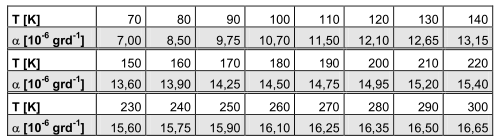
\includegraphics[width=0.7\textwidth]{alpha.PNG}
  \caption{Linearer Ausdehnungskoeffizient von Kupfer in Abhängigkeit von der Temperatur.}
  \label{fig:alpha}
\end{figure}

Die Tabelle \ref{tab:C_P_C_V} enthält die berechneten Werte von $C_p$ nach Gleichung \eqref{eqn:C_p} und $C_V$ nach Gleichung \eqref{eqn:C_V}.
Wobei für die Temperatur bei der $C_V$ Berechnung ein $T_{mittel}$ verwendet wird, was sich aus den Temperaturen $T_{probe}$ aus Tabelle \ref{tab:Messwerte}
mit der Gleichung
\begin{align}
  T_{mittel} = T_1 + \frac{T_2-T_1}{2} \pm \frac{T_2-T_1}{2}
\end{align}
ergibt.

\begin{table}  %   Messwerte_C_P_C_V
  \centering
  \caption{.}
  \label{tab:C_P_C_V}
  \begin{tabular}{c c c c c c}
    \toprule
    $\Delta t/\si{\second}$ & $\Delta T/ \si{\kelvin}$ & $C_p$ & $T_{mittel}$ & $\alpha$ & $C_V$\\
    \midrule
    150	&	5.2	&	13.02	\pm	0.44	&	88.1	\pm	2.6	&	9.44	\pm0.29	&	12.95	\pm 0.44   \\
    150	&	4.7	&	14.29	\pm	0.48	&	93.1	\pm	2.4	&	9.97	\pm0.24	&	14.20	\pm 0.48   \\
    150	&	3.6	&	19.01	\pm	0.64	&	97.2	\pm	1.8	&	10.38	\pm	0.17	&	18.92	\pm	0.64   \\
    150	&	4.3	&	15.81	\pm	0.54	&	101.2	\pm	2.1	&	10.74	\pm	0.19	&	15.71	\pm	0.54   \\
    150	&	4.5	&	14.95	\pm	0.51	&	105.6	\pm	2.3	&	11.11	\pm	0.18	&	14.83	\pm	0.51   \\
    150	&	4.5	&	14.92	\pm	0.51	&	110.1	\pm	2.3	&	11.47	\pm	0.17	&	14.79	\pm	0.51   \\
    150	&	4.5	&	14.89	\pm	0.50	&	114.6	\pm	2.3	&	11.79	\pm	0.16	&	14.74	\pm	0.50   \\
    150	&	4.1	&	16.60	\pm	0.56	&	118.9	\pm	2.0	&	12.08	\pm	0.13	&	16.45	\pm	0.56   \\
    150	&	3.8	&	17.61	\pm	0.60	&	122.9	\pm	1.9	&	12.33	\pm	0.11	&	17.44	\pm	0.60   \\
    150	&	7.5	&	9.06	\pm	0.31	&	128.6	\pm	3.7	&	12.65	\pm	0.20	&	8.88	\pm 0.31   \\
    300	&	6.8	&	20.01	\pm	0.68	&	135.7	\pm	3.4	&	13.00	\pm	0.16	&	19.80	\pm	0.68   \\
    300	&	6.5	&	20.69	\pm	0.70	&	142.3	\pm	3.3	&	13.30	\pm	0.14	&	20.46	\pm	0.70   \\
    300	&	7.0	&	19.20	\pm	0.65	&	149.1	\pm	3.5	&	13.57	\pm	0.13	&	18.95	\pm	0.65   \\
    300	&	6.6	&	20.56	\pm	0.70	&	155.9	\pm	3.3	&	13.81	\pm	0.11	&	20.29	\pm	0.70   \\
    300	&	6.1	&	22.14	\pm	0.75	&	162.3	\pm	3.1	&	14.02	\pm	0.09	&	21.86	\pm	0.75   \\
    300	&	5.9	&	23.00	\pm	0.78	&	168.3	\pm	2.9	&	14.19	\pm	0.08	&	22.70	\pm	0.78   \\
    300	&	6.4	&	21.18	\pm	0.72	&	174.4	\pm	3.2	&	14.36	\pm	0.08	&	20.85	\pm	0.72   \\
    300	&	6.2	&	21.96	\pm	0.74	&	180.7	\pm	3.1	&	14.51	\pm	0.08	&	21.62	\pm	0.74   \\
    300	&	6.4	&	21.06	\pm	0.71	&	187.0	\pm	3.2	&	14.66	\pm	0.07	&	20.70	\pm	0.71   \\
    300	&	6.7	&	20.22	\pm	0.69	&	193.5	\pm	3.3	&	14.81	\pm	0.07	&	19.84	\pm	0.69   \\
    300	&	5.7	&	23.67	\pm	0.80	&	199.7	\pm	2.9	&	14.94	\pm	0.06	&	23.28	\pm	0.80   \\
    300	&	5.7	&	23.62	\pm	0.80	&	205.4	\pm	2.9	&	15.06	\pm	0.06	&	23.20	\pm	0.80   \\
    300	&	6.2	&	21.67	\pm	0.73	&	211.4	\pm	3.1	&	15.19	\pm	0.06	&	21.23	\pm	0.73   \\
    300	&	12.5&	10.79 \pm	0.37	&	220.8	\pm	6.3	&	15.37	\pm	0.12	&	10.33	\pm	0.37   \\
    300	&	5.8	&	23.37	\pm	0.79	&	230.0	\pm	2.9	&	15.55	\pm	0.06	&	22.87	\pm	0.79   \\
    300	&	6.1	&	22.34	\pm	0.76	&	235.9	\pm	3.0	&	15.67	\pm	0.06	&	21.82	\pm	0.76   \\
    300	&	6.6	&	20.57	\pm	0.70	&	242.2	\pm	3.3	&	15.79	\pm	0.06	&	20.03	\pm	0.70   \\
    300	&	5.1	&	26.68	\pm	0.90	&	248.1	\pm	2.5	&	15.90	\pm	0.05	&	26.11	\pm	0.90   \\
    300	&	5.3	&	25.35	\pm	0.86	&	253.3	\pm	2.7	&	15.99	\pm	0.05	&	24.77	\pm	0.86   \\
    300	&	5.9	&	23.09	\pm	0.78	&	258.9	\pm	2.9	&	16.09	\pm	0.05	&	22.49	\pm	0.78   \\
    300	&	7.7	&	17.66	\pm	0.60	&	265.6	\pm	3.8	&	16.20	\pm	0.06	&	17.03	\pm	0.60   \\
    300	&	4.6	&	29.35	\pm	1.00	&	271.8	\pm	2.3	&	16.30	\pm	0.03	&	28.71	\pm	1.00   \\
    300	&	5.6	&	23.97	\pm	0.81	&	276.9	\pm	2.8	&	16.37	\pm	0.04	&	23.30	\pm	0.81   \\
    300	&	6.2	&	21.92	\pm	0.74	&	282.8	\pm	3.1	&	16.45	\pm	0.04	&	21.23	\pm	0.74   \\
    300	&	5.7	&	23.85	\pm	0.81	&	288.7	\pm	2.8	&	16.51	\pm	0.03	&	23.15	\pm	0.81   \\
    300	&	5.9	&	22.76	\pm	0.77	&	294.5	\pm	3.0	&	16.56	\pm	0.02	&	22.04	\pm	0.77   \\
    \bottomrule
  \end{tabular}
\end{table}

Um aus den berechneten $C_V$ aus Tabelle \ref{tab:C_P_C_V} die Debyetemperatur $\theta_D$ von Kupfer zu bestimmen,
wird an die Werte der Debyefunktion, die in Tabelle \ref{fig:debye} aufgetragen sind,
eine Funktion der Form
\begin{align}
 \frac{\theta_D}{T} = f(C_V) =  a C_V^4 + b  C_V^3 + c C_V^2 + d C_V + f + \frac{x}{C_V}
\end{align}
gefittet.

\begin{figure}
 \centering
 \includegraphics{width=0.7\textwidth}{Debye.PNG}
   \caption{Werte für die Debyefunktion.}
   \label{fig:debye}
 \end{figure}



Die Debyetemperatur $\theta_D$ ergibt sich somit aus
\begin{align}
  \theta_D = \frac{f(C_V(T))}{T}. \label{eqn:theta_D}
\end{align}
Wobei nur Messwerte von $C_V(T)$ bis zur einer Temperatur $T_{max}=\SI{170}{\kelvin} $ benutzt werden.
Die Tabelle \ref{tab:Debyetemperatur} enthält alle
Temperatur bis zur Temperatur $T_{max}$ und die nach Gleichung \eqref{eqn:theta_D}
bestimmte Debyetemperatur $\theta_D$.

\begin{table}
  \centering
  \caption{}
  \label{tab:Debyetemperatur}
  \begin{tabular}{c c c c}
\toprule
$C_V/ $ &  $ \theta_D/T $   &   T/ $\si{\kelvin}$  & $\theta_D/\si{\kelvin}$  \\
\midrule
12.95	\pm	0.44	&	3.93	\pm	0.10	&	88.1	\pm	2.6	&	346.4	\pm	13.6   \\
14.20	\pm	0.48	&	3.65	\pm	0.11	&	93.1	\pm	2.4	&	339.8	\pm	13.3   \\
15.71	\pm	0.54	&	3.31	\pm	0.12	&	101.2	\pm	2.1	&	334.7	\pm	14.5   \\
14.83	\pm	0.51	&	3.51	\pm	0.11	&	105.6	\pm	2.3	&	370.4	\pm	14.5   \\
14.79	\pm	0.51	&	3.52	\pm	0.11	&	110.1	\pm	2.3	&	387.4	\pm	15.0   \\
14.74	\pm	0.50	&	3.53	\pm	0.11	&	114.6	\pm	2.3	&	404.5	\pm	15.4   \\
16.45	\pm	0.56	&	3.13	\pm	0.14	&	118.9	\pm	2.0	&	372.6	\pm	17.5   \\
17.44	\pm	0.60	&	2.88	\pm	0.15	&	122.9	\pm	1.9	&	354.5	\pm	19.8   \\
19.80	\pm	0.68	&	2.22	\pm	0.21	&	135.7	\pm	3.4	&	301.3	\pm	29.3   \\
20.46	\pm	0.70	&	2.01	\pm	0.23	&	142.3	\pm	3.3	&	286.7	\pm	32.8   \\
18.95	\pm	0.65	&	2.47	\pm	0.19	&	149.1	\pm	3.5	&	368.7	\pm	29.4   \\
20.29	\pm	0.70	&	2.07	\pm	0.22	&	155.9	\pm	3.3	&	322.5	\pm	35.2   \\
21.86	\pm	0.75	&	1.55	\pm	0.26	&	162.3	\pm	3.1	&	250.7	\pm	43.2   \\
22.70	\pm	0.78	&	1.24	\pm	0.29	&	168.3	\pm	2.9	&	208.8	\pm	48.7   \\
\bottomrule
\end{tabular}
\end{table}

Als Mittelwert ergibt sich aus den Werten aus der Tabelle \ref{tab:Debyetemperatur}
für die Debyetemperatur von Kupfer
\begin{align}
\theta_{D_{Kupfer}} = \SI{332(52)}{\kelvin} .
\end{align}


\subsection{Theoriewert der Debyetemperatur}
\label{subsec:theoriewert}

Aus der Gleichung
\begin{align}
  \int_0^{\omega_D} z(\omega)\text{d}\omega = 3 N_L
\end{align}
ergibt sich die Debyefrequenz $\omega_D$ zu
\begin{align}
  \omega_D^3 = \frac{18\pi^2 N_L}{L^3} \frac{1}{\left(\frac{1}{v_l^3}+\frac{2}{v_{tr}^3\right)}} \label{eqn:5}
\end{align}
mit dem Probevolumen $L^3$ und der Teilchenzahl in der Probe $N_L$.
Das Probevolumen ergibt sich über die Masse der Probe $m=\SI{}{\kilo\gram}$ und der Dichte von Kupfer $\rho=\SI{8.96e3}{\kilo\gram\per\cubic\meter}$
zu $L^3=m\rho$.
Über die Molaremasse von Kupfer $M=\SI{63.546e-3}{\kilo\gram\per\mol}$ und die Avogadrokonstante $N_A$ berechnet sich die
Teilchenzahl zu
$N_L=\frac{m N_A}{M}$.
Nach Gleichung \eqref{eqn:5} folgt somit
für die theoretische
Debyefrequenz
\begin{align}
  \omega_D &= \SI{4.35e13}{\hertz}.
\intertext{Über den Zusammenhang}
  \theta_{D} &= \frac{\hbar \omega_D}{k_B}
\intertext{folgt für die theoretische Debyetemperatur }
\theta_D &= \SI{332.5}{\kelvin}.
\end{align}


\section{Diskussion}
\label{sec:Diskussion}
In Tabelle \ref{tab:vergleiche} sind die
bestimmten Werte für Elektronendichte $\rho$ und $\delta$ und Literaturwerte und die
relative Abweichung gezeigt.
\begin{table}
  \caption{Bestimmte Werte für $\rho$ und $\delta = n - 1$
  der Schicht(PS) und dem Substrat(Silizium) im Vergleich mit Literaturwerten.}
  \label{tab:vergleiche}
  \begin{tabular}{l l l l}
      \toprule
       Messgröße & Messwerte & Literaturwerte \cite{sample} & rel. Abweichung \\
       \midrule
       $\rho_\text{PS} \text{ in } \si{\per\cubic\meter}$ & $\num{3.13(4)e29} $ & \num{3.371e29} & \SI{7(1)}{\percent} \\
       $\rho_\text{Silizium} \text{ in } \si{\per\cubic\meter}$ & \num{6.89(4)e29} & \num{7.097e29} & \SI{3(1)}{\percent} \\
       $\delta_\text{PS} $  & $\num{3.33(4)e-6}$ & $\num{3.5e-6}$  & $ \SI{5(1)}{\percent} $ \\
       $\delta_\text{Silizium}$ & $ \num{7.33(4)e-6} $ & $\num{7.6e-6}$  & $ \SI{4(1)}{\percent} $ \\
      \bottomrule
  \end{tabular}
\end{table}
Die sich ergebendenen relativen Abweichungen zu den Literaturwerten aus Tabelle \ref{tab:vergleiche}
sind zu groß, um von einer genauen Messung auszugehen.
Mögliche Ursachen liegen zum einen an der Anzahl der Freiheitsgerade
bei dem Fit mit dem modifizierten Parrat Algorithmus. Um bessere Ergebnisse
zu erhalten könnte noch in Erwägung gezogen werden, die verschiedenen Bereiche
im Fit gesondert zu gewichten. So könnten relevantere Bereiche besonders
berücksichtigt werden.

Für die Rauigkeit der Polystyrolschicht wurde ein Wert von $ \SI{{17.9(5)e-10}}{} $
und für die
Rauigkeit des Wafers ein Wert von $ \SI{4.53(7)e-10}{} $gemesen. Auffällig ist
der große Fehler auf die Rauigkeit der Polystyrolschicht, sodass der gemessene Wert
nicht besonders aussagekräftig ist.

In Abbildung \ref{fig:messung} wird deutlich, dass wenn für
Elektronendichten und Brechungsindizes die Literaturwerte eingesetzt werden
und als freie Parameter die Rauigkeit und der z-Wert übrig bleiben, keine
gute Anpassung an die Messwerte erreicht wird.
Somit lässt sich vermuten, dass ein systematischer Fehler bezüglich des
Messvorgangs vorliegt.

\FloatBarrier
\begin{figure}
 \centering
   \includegraphics[width=0.7\textwidth]{build/Programm_mit_lit.pdf}
   \caption{Normierte Reflektivität $R$ gegen den Einfallswinkel $\alpha_i$ aufgetragen und
    Fit an die markierten Messwerte. Sowie eine Reflektivitätskurve mit den Literaturwerten der Dispersionen und angepasster Rauigkeit.}
   \label{fig:messung}
\end{figure}
\FloatBarrier

Abschließend lässt sich sagen, dass bei der durchgeführten Messung, zwar
der erwartete Zusammenhang visuell bestätigt werden konnte, allerdings die
Anpassung an die Messwerte Parameter liefert die stark von den Literaturwerten
Abweichung beziehungsweise einen großen Fehler aufweisen.
Dabei ist zu bemerken, dass die verschiedenen Justageschritte viel Potenzial
für sytematische Fehler beherbergen.


% Korrektur durch Geometriefaktor <-- Hier zu was schreiben

%  -> Fit Detektorscan

%  -> Fit Rockingscan 0 grad

%   -> Korrektur


% Bestimmung der Parameter

%  -> Schichtdicke

%  -> Rauigkeit  <--- Hier zu was schreiben

%  -> Elektronendichte

% -zuviele Fitparameter um eine Genaue Anpassung zu erhalten
%  je nachdem ob an log gefittet wurde oder nicht andere Ergebnisse
%
% - Rockingscan und Detektorscan liefern gewünschte Ergebnisse
%
% - diffuse_Scan nicht wirklicher untergrund aber nur gerninge auswirkung auf den verlauf so
% wie der Gemometrie faktor


\printbibliography

\newpage

\section{Anhang}
\begin{figure}
  \centering
  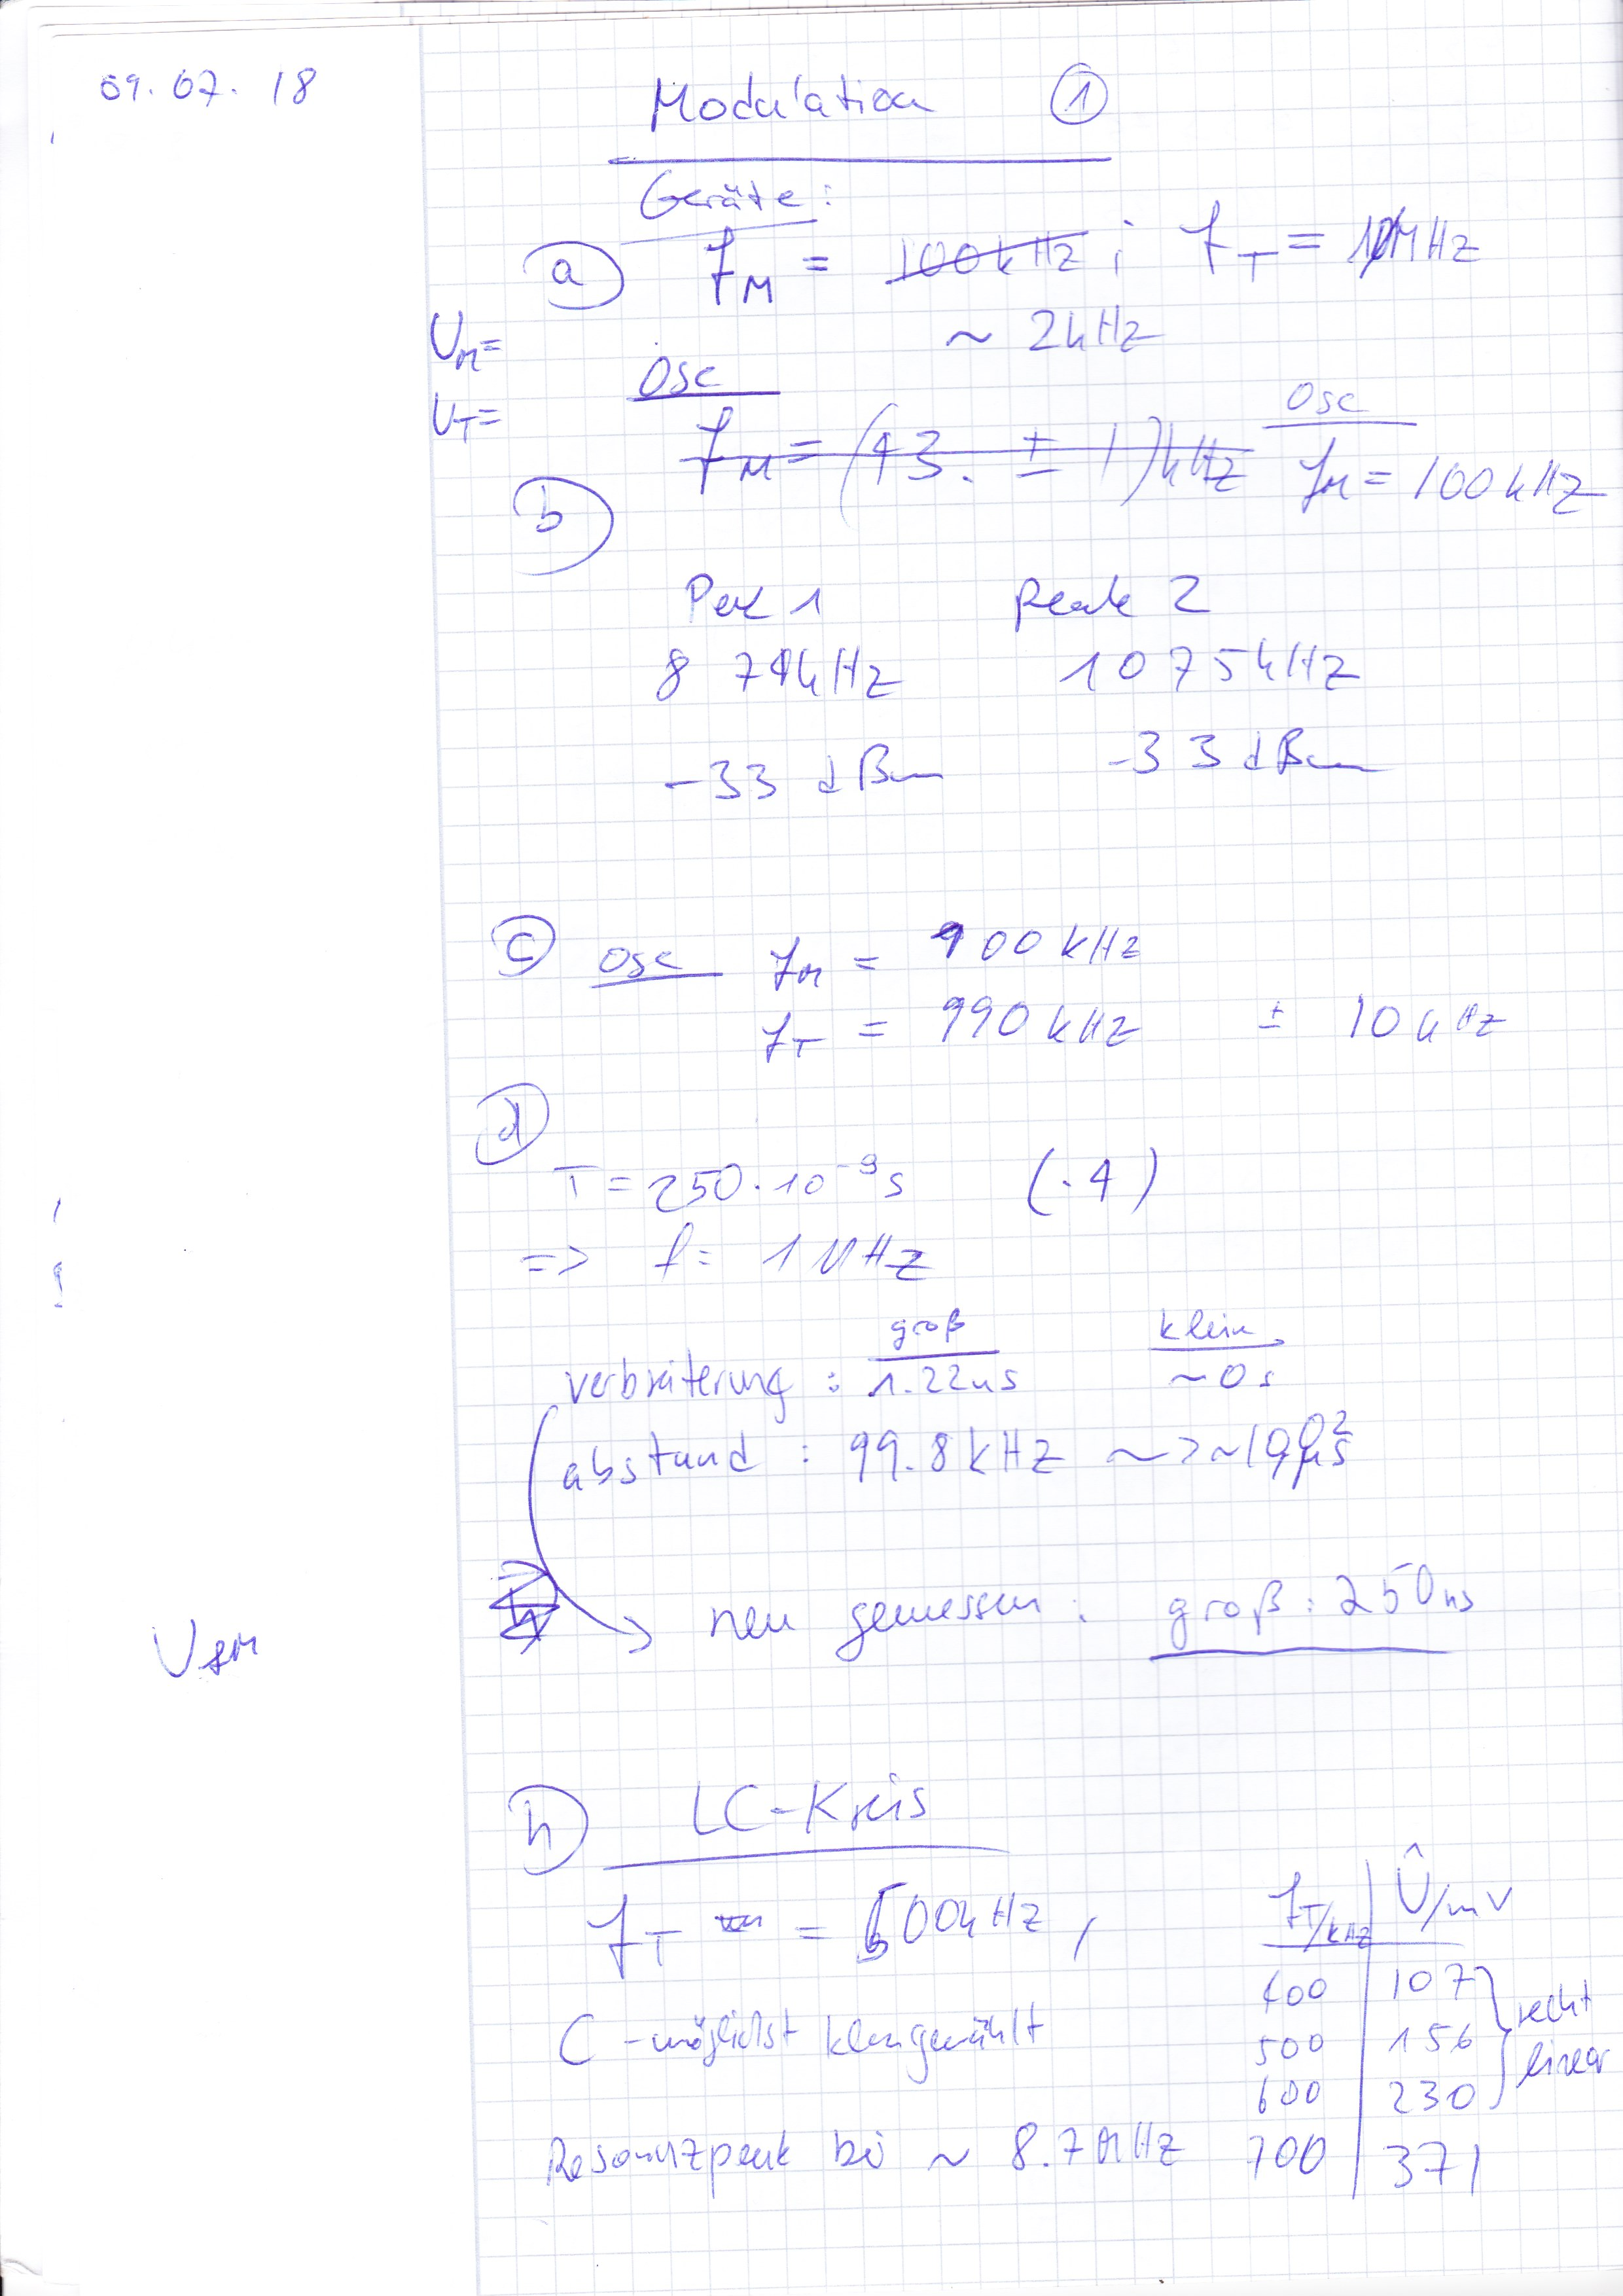
\includegraphics[width=0.95\textwidth]{messheft/seite_1.jpg}
  \caption{}
\label{fig:p1}
\end{figure}

\FloatBarrier
\begin{figure}
  \centering
  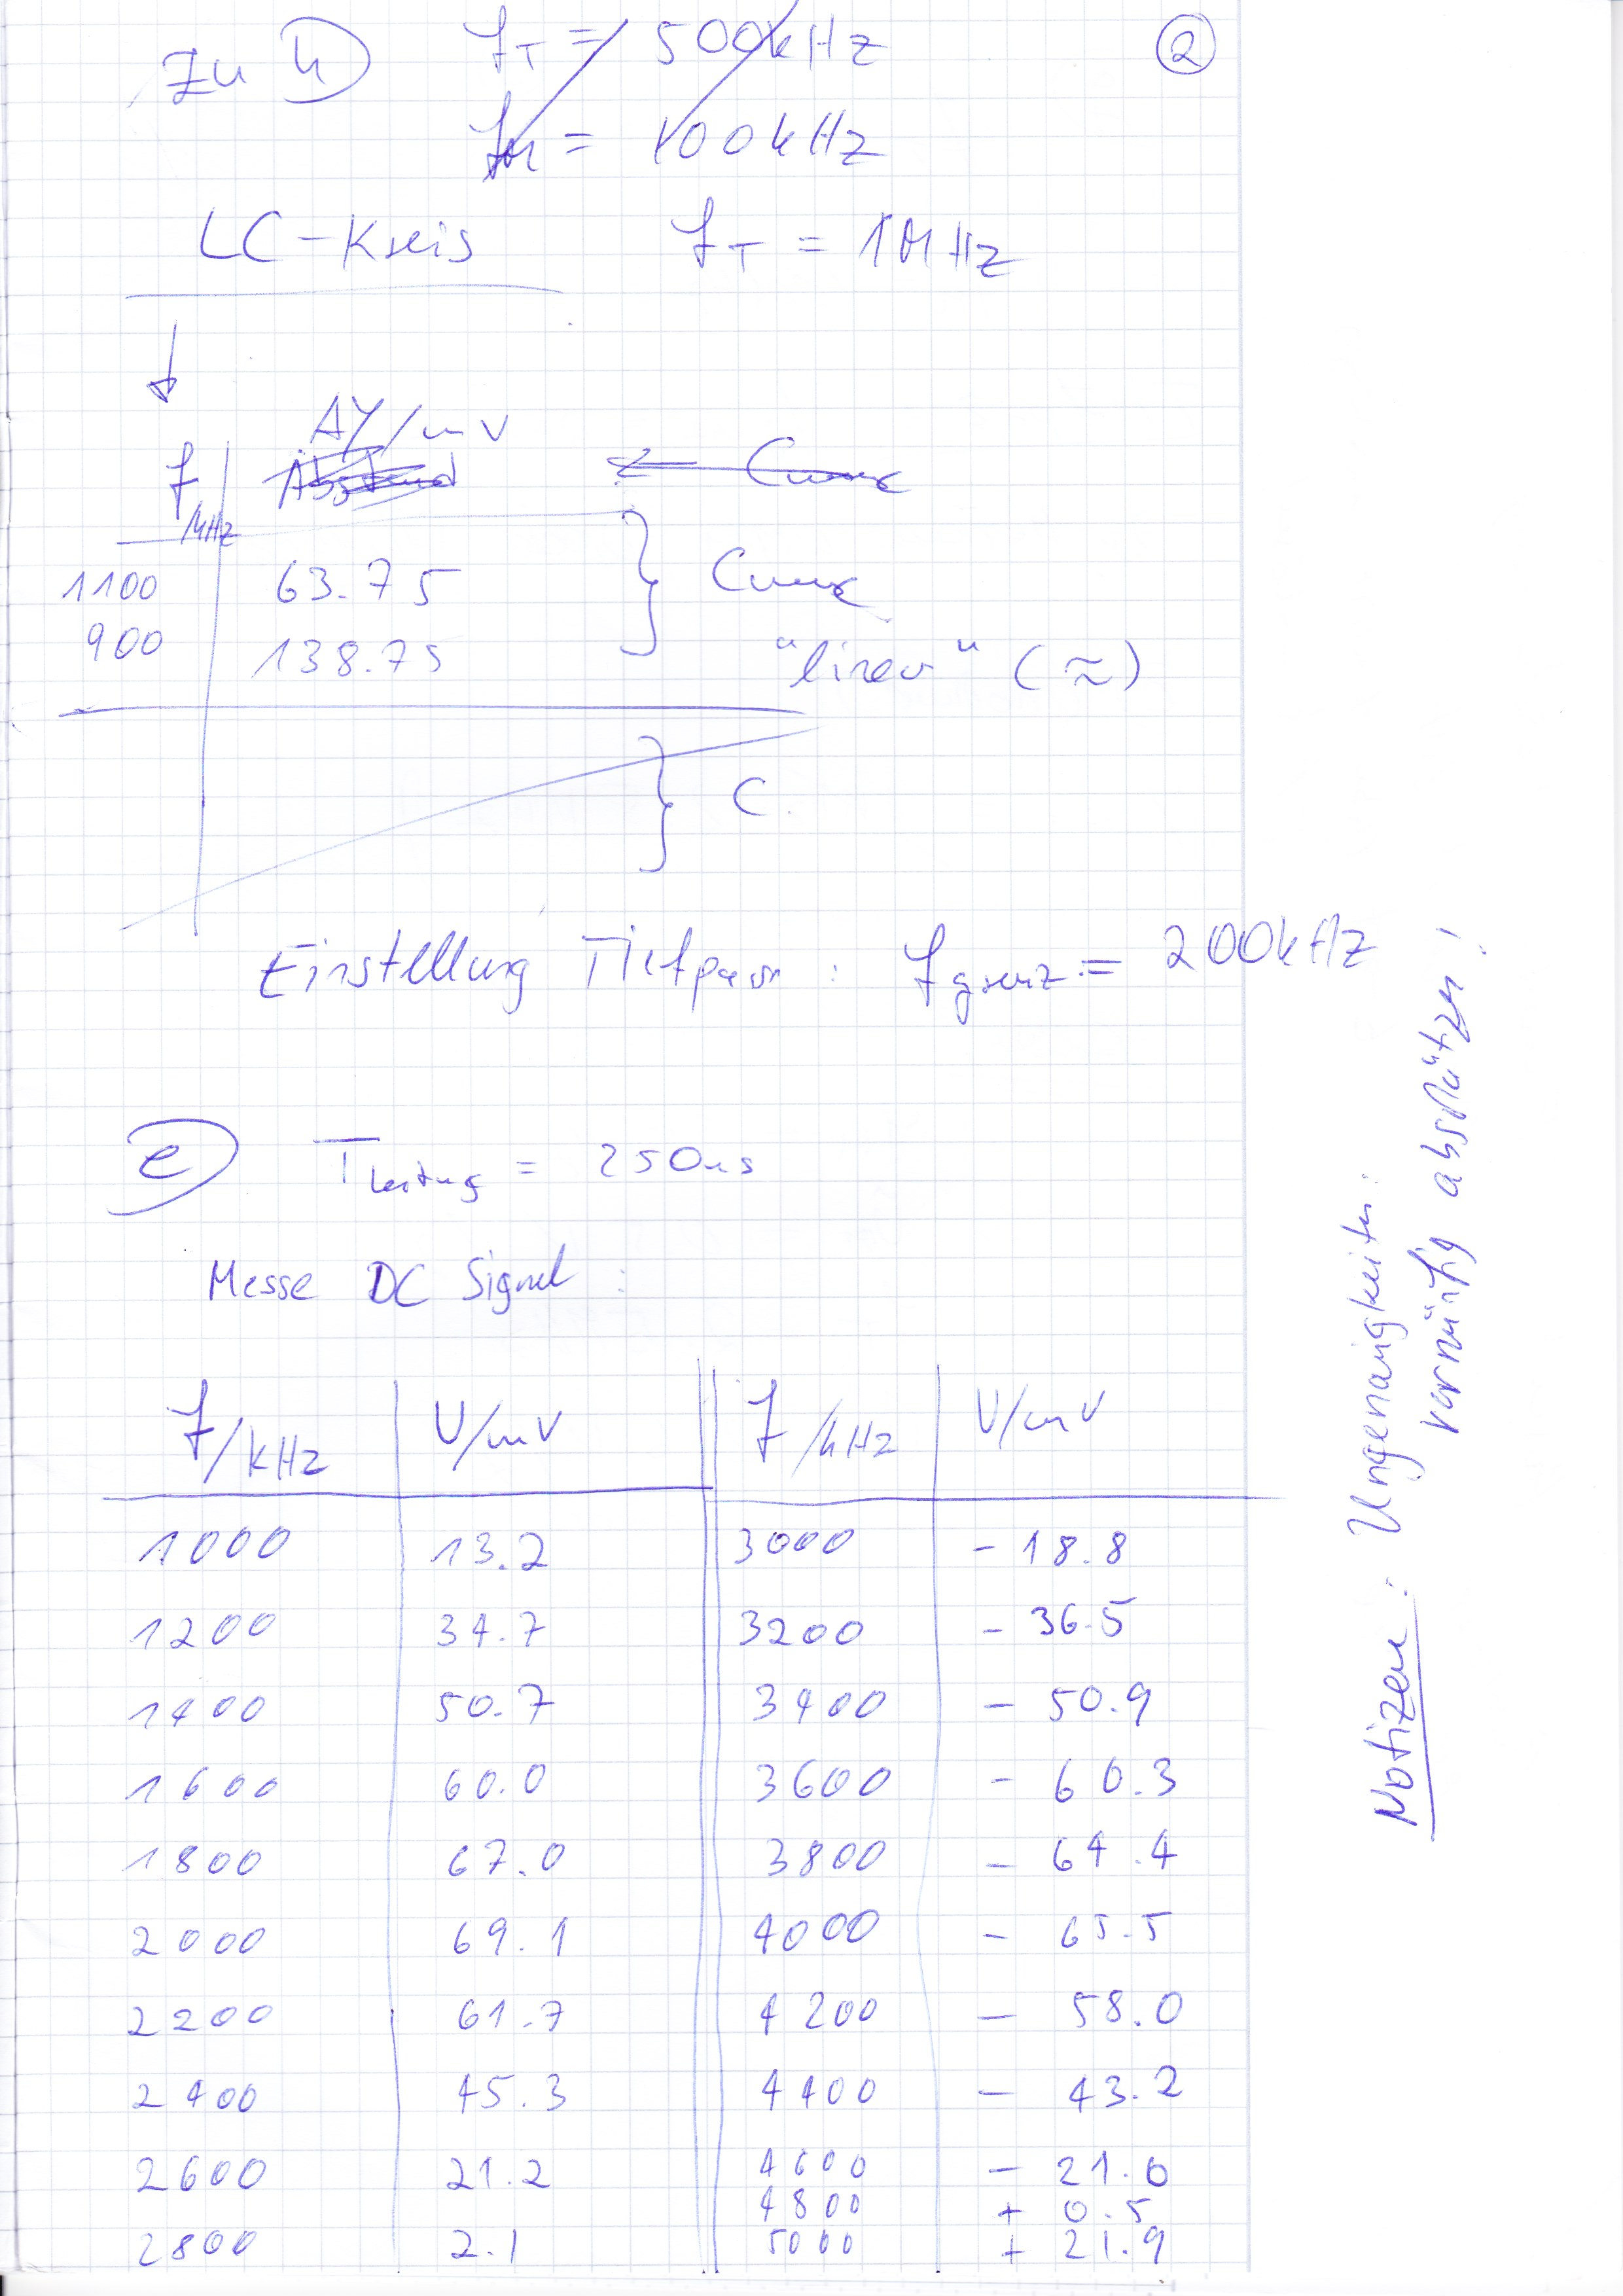
\includegraphics[width=0.95\textwidth]{messheft/seite_2.jpg}
  \caption{}
\label{fig:p2}
\end{figure}

\FloatBarrier
\begin{figure}
  \centering
  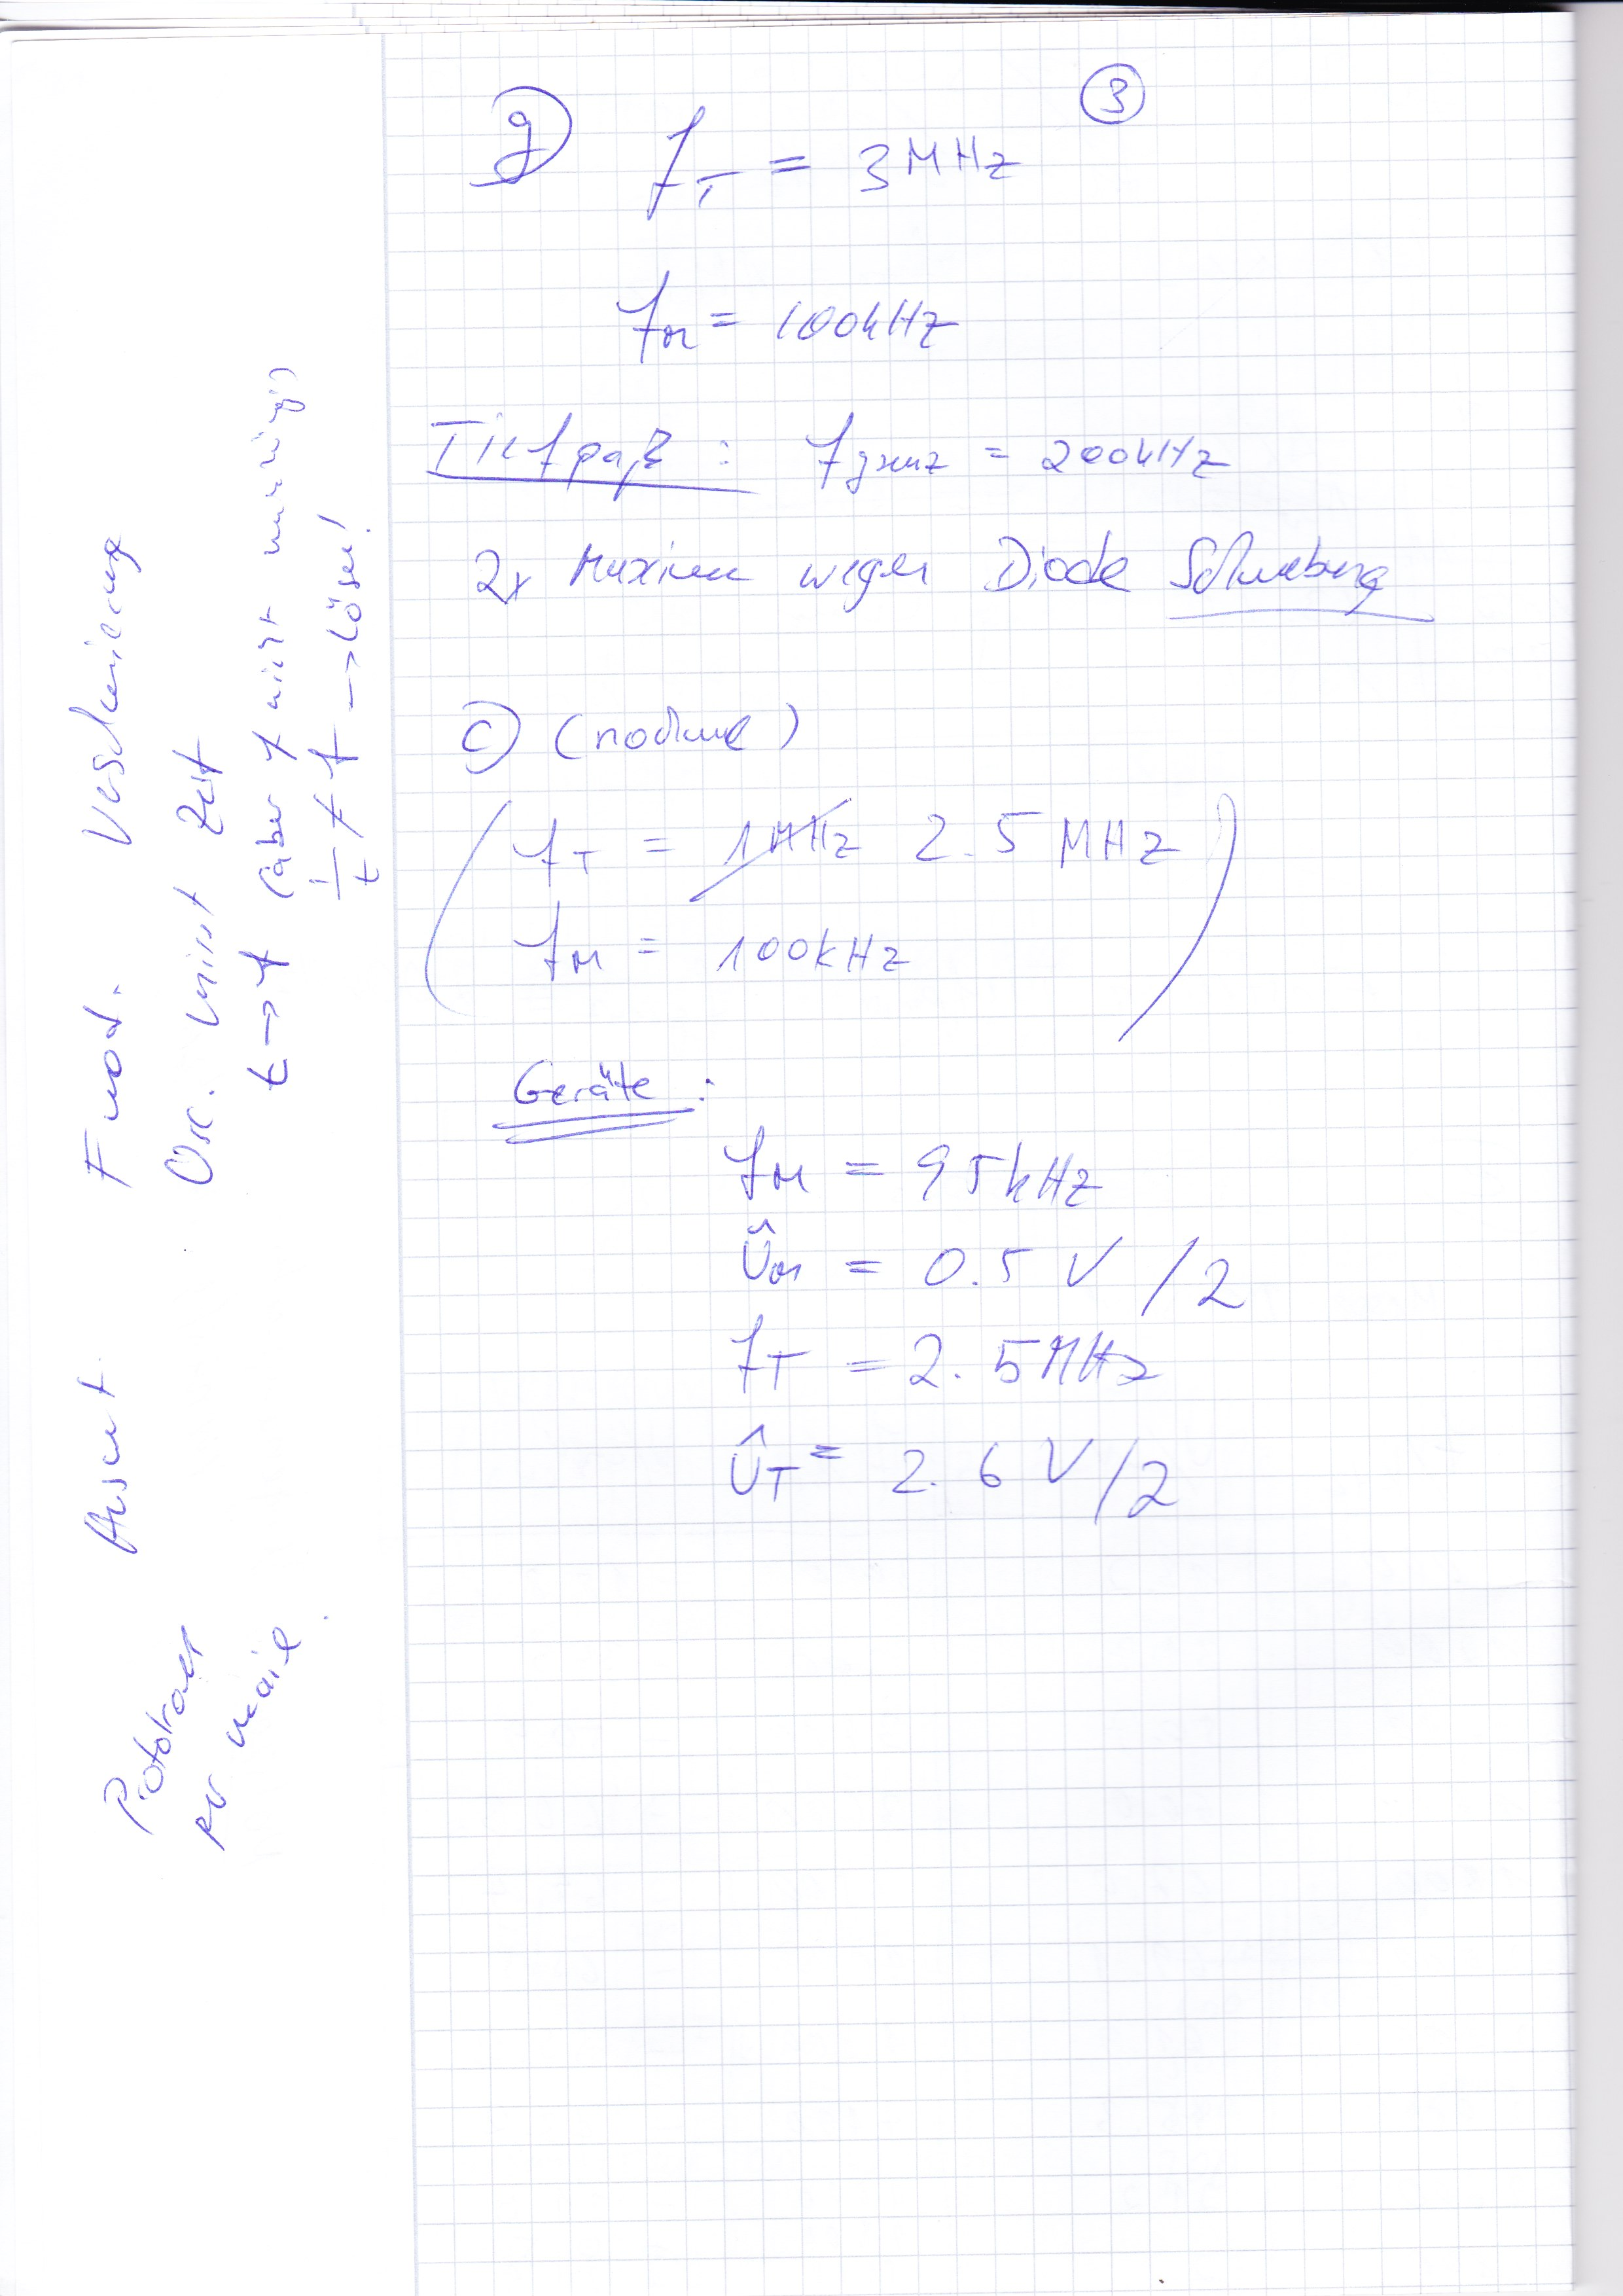
\includegraphics[width=0.95\textwidth]{messheft/seite_3.jpg}
  \caption{}
\label{fig:p3}
\end{figure}
\end{document}
